\documentclass[12pt,fleqn]{article}
\setlength{\parindent}{0pt}
\usepackage{graphicx}
\usepackage{cancel}
\usepackage{listings}
\usepackage[latin5]{inputenc}
\usepackage{color}
\setlength{\parskip}{8pt}
\setlength{\parsep}{0pt}
\setlength{\headsep}{0pt}
\setlength{\topskip}{0pt}
\setlength{\topmargin}{0pt}
\setlength{\topsep}{0pt}
\setlength{\partopsep}{0pt}
\setlength{\mathindent}{0cm}
\usepackage{latexsym}
\usepackage{showkeys}
\renewcommand*\showkeyslabelformat[1]{(#1)}

\begin{document}
Ders 22

Muhendislerin Laplace Transformunu sevmesinin sebeplerinden biri
fonksiyonlarda kesintili / birdenbire ziplayan gecisleri (jump
discontinuities) durumlarinda bozulmadan isleyebiliyor olmasidir. 

Kesintili fonksiyonlardan biri birim adim fonksiyonudur. Fonksiyonun
kendisi tartisma yaratan bir fonksiyon aslinda, sifir noktasinda hangi
degere sahip oldugu hala kararlastirilamadi. Bazilari 0 diyor, bazilari 1
diyor, ben bu derste tanimsiz birakacagim. 

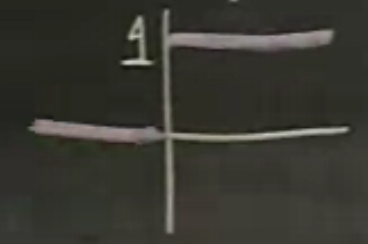
\includegraphics[height=3cm]{22_1.png}




\end{document}
